\begin{frame}[t]
  \frametitle{Spin-orbit coupling}
  \small
  Our original Hamiltonian
  \[
  H = \sum_{i=1}^N \left[ -\frac{1}{2} \nabla_i^2 - \frac{Z}{r_i} \right] + \sum_{i<j}^N \frac{1}{|\vec{r}_i - \vec{r}_j|}
  \] \pause
  A \emph{magnetic} force?
  \vspace{-1em}
  \begin{center}
  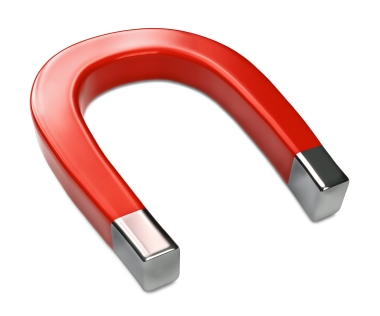
\includegraphics[width=0.4\textwidth]{magnet}
  \end{center}
\end{frame}

\begin{frame}[t]
  \frametitle{Spin-orbit coupling}
  \small
  The Hamiltonian with \emph{spin-orbit} effect
  \[
  H = \sum_{i=1}^N \left[ -\frac{1}{2} \nabla_i^2 - \frac{Z}{r_i} \right] + \sum_{i<j}^N \frac{1}{|\vec{r}_i - \vec{r}_j|} + \underbrace{\sum_{i=1}^N \xi(r_i) \boldsymbol{\ell}_i\cdot\vec{s}_i}_{\emph{\text{Weak}}}
  \]
  where,
  \[ \xi(r) = \frac{1}{2c^2} \frac{1}{r} \frac{dV}{dr} \]
  In atomic units
  \[ c \approx 137.036\ \mathrm{a_0/t_0} \]
\end{frame}

\begin{frame}[t]
  \frametitle{Spin-orbit coupling within multiplet terms}
  \small
  \emph{Clebsch-Grodan} transformation
  \[ \Ket{L,M_L,S,M_S} \rightarrow \Ket{L,S,J,M_J} \]
  Multiplet split
  \[ ^{2S+1}L_J \quad \text{with} \quad J=L+S,L+S-1,\ldots,|L-S| \]
  \[ ^3P \rightarrow {^3P_2},{^3P_1},{^3P_0} \]
  Eigen-energies
  \[\boxed{
  E_\text{SO} = A(nl,LS) \frac{1}{2}[J(J+1)-L(L+1)-S(S+1)]
  }\]
\end{frame}

\begin{frame}[t]
  \frametitle{Spin-orbit coupling within multiplet terms}
  \footnotesize
  Energy splitting
  \vspace{-2em}
  \begin{figure}[h!]
  \begin{center}
  \begin{tikzpicture}[scale=0.12]
  \newcommand{\LA}{0}
  \newcommand{\RA}{15}
  \newcommand{\LB}{30}
  \newcommand{\RB}{45}
  \newcommand{\LC}{60}
  \newcommand{\RC}{75}
  \newcommand{\EA}{13.7797}
  \newcommand{\EBa}{27.5594}
  \newcommand{\EBb}{11.0236}
  \newcommand{\EBc}{0}
  \newcommand{\ECa}{27.5594}
  \newcommand{\ECb}{11.0236}
  \newcommand{\ECc}{ 4.36}
  \newcommand{\ECd}{-4.36}
  \newcommand{\ECe}{-8.72}
  %
  \draw[very thick] (\LA,\EA) -- (\RA,\EA);
  %
  \draw[very thick] (\LB,\EBa) -- (\RB,\EBa);
  \draw[very thick] (\LB,\EBb) -- (\RB,\EBb);
  \draw[very thick] (\LB,\EBc) -- (\RB,\EBc);
  %
  \draw[very thick] (\LC,\ECa) -- (\RC,\ECa);
  \draw[very thick] (\LC,\ECb) -- (\RC,\ECb);
  \draw[very thick] (\LC,\ECc) -- (\RC,\ECc);
  \draw[very thick] (\LC,\ECd) -- (\RC,\ECd);
  \draw[very thick] (\LC,\ECe) -- (\RC,\ECe);
  %
  \node at (\LA+8,\EA+2) {$p^2$};
  \node at (\LB+7,\EBa+2) {$^1S$};
  \node at (\LB+7,\EBb+2) {$^1D$};
  \node at (\LB+7,\EBc+2) {$^3P$};
  \node at (\LC+7,\ECa+2) {$^1S_0$};
  \node at (\LC+7,\ECb+2) {$^1D_2$};
  \node at (\LC+7,\ECc+2) {$^3P_2$};
  \node at (\LC+7,\ECd+2) {$^3P_1$};
  \node at (\LC+7,\ECe+2) {$^3P_0$};
  %
  \draw[very thin, gray, dashed] (\RA,\EA) -- (\LB,\EBa);
  \draw[very thin, gray, dashed] (\RA,\EA) -- (\LB,\EBb);
  \draw[very thin, gray, dashed] (\RA,\EA) -- (\LB,\EBc);
  %
  \draw[very thin, gray, dashed] (\RB,\EBa) -- (\LC,\ECa);
  \draw[very thin, gray, dashed] (\RB,\EBb) -- (\LC,\ECb);
  \draw[very thin, gray, dashed] (\RB,\EBc) -- (\LC,\ECc);
  \draw[very thin, gray, dashed] (\RB,\EBc) -- (\LC,\ECd);
  \draw[very thin, gray, dashed] (\RB,\EBc) -- (\LC,\ECe);
  %
  \draw[triangle 45-triangle 45] (\LB+12,\EBa) -- (\LB+12,\EBb);
  \draw[triangle 45-triangle 45] (\LB+12,\EBa) -- (\LB+12,\EBc);
  \draw[triangle 45-triangle 45] (\LC+12,\ECc) -- (\LC+12,\ECd);
  \draw[triangle 45-triangle 45] (\LC+12,\ECd) -- (\LC+12,\ECe);
  %
  \node at (\RB+7,19.2915) {$\Delta E = 0.082679$};
  \node at (\RB+7,5.5118) {$\Delta E = 0.055118$};
  \node at (\RC+7,0) {$\Delta E = 0.000218$};
  \node at (\RC+7,-6.54) {$\Delta E = 0.000109$};
  %
  \node at (\LA+7.5,-14) {Configuration};
  \node at (\LB+7.5,-14) {Coulomb repulsion};
  \node at (\LC+7.5,-14) {Spin-orbit};
  \end{tikzpicture}
  \end{center}
  \end{figure}
  
  \pause \Put(195,110){
\includegraphics[width=0.55\textwidth]{mag}}
\end{frame}

\begin{frame}[t]
  \frametitle{Spin-orbit coupling within entire shell}
  \footnotesize
  \begin{center}
  \vspace{-0.5em}
  \begin{tabular}{|c|c|c|}
  \hline
  $\bullet$ & $\bullet$ & $\phantom{\bullet}$ \\ \hline
  &  &  \\
  \hline
  \end{tabular}
  \begin{tabular}{|c|c|c|}
  \hline
  $\bullet$ & $\phantom{\bullet}$ & $\bullet$ \\ \hline
  &  &  \\
  \hline
  \end{tabular}
  \begin{tabular}{|c|c|c|}
  \hline
  $\bullet$ & $\phantom{\bullet}$ & $\phantom{\bullet}$ \\ \hline
  $\bullet$ &  &  \\
  \hline
  \end{tabular}
  \begin{tabular}{|c|c|c|}
  \hline
  $\bullet$ & $\phantom{\bullet}$ & $\phantom{\bullet}$ \\ \hline
  & $\bullet$ &  \\
  \hline
  \end{tabular}
  \begin{tabular}{|c|c|c|}
  \hline
  $\bullet$ & $\phantom{\bullet}$ & $\phantom{\bullet}$ \\ \hline
  &  & $\bullet$ \\
  \hline
  \end{tabular} \\
  \vspace{0.5em}
  \begin{tabular}{|c|c|c|}
  \hline
  $\phantom{\bullet}$ & $\bullet$ & $\bullet$ \\ \hline
  &  &  \\
  \hline
  \end{tabular}
  \begin{tabular}{|c|c|c|}
  \hline
  $\phantom{\bullet}$ & $\bullet$ & $\phantom{\bullet}$ \\ \hline
  $\bullet$ &  &  \\
  \hline
  \end{tabular}
  \begin{tabular}{|c|c|c|}
  \hline
  $\phantom{\bullet}$ & $\bullet$ & $\phantom{\bullet}$ \\ \hline
  & $\bullet$ &  \\
  \hline
  \end{tabular}
  \begin{tabular}{|c|c|c|}
  \hline
  $\phantom{\bullet}$ & $\bullet$ & $\phantom{\bullet}$ \\ \hline
  &  & $\bullet$ \\
  \hline
  \end{tabular}
  \begin{tabular}{|c|c|c|}
  \hline
  $\phantom{\bullet}$ & $\phantom{\bullet}$ & $\bullet$ \\ \hline
  $\bullet$ &  &  \\
  \hline
  \end{tabular} \\
  \vspace{0.5em}
  \begin{tabular}{|c|c|c|}
  \hline
  $\phantom{\bullet}$ & $\phantom{\bullet}$ & $\bullet$ \\ \hline
  & $\bullet$ &  \\
  \hline
  \end{tabular}
  \begin{tabular}{|c|c|c|}
  \hline
  $\phantom{\bullet}$ & $\phantom{\bullet}$ & $\bullet$ \\ \hline
  &  & $\bullet$ \\
  \hline
  \end{tabular}
  \begin{tabular}{|c|c|c|}
  \hline
  $\phantom{\bullet}$ & $\phantom{\bullet}$ & $\phantom{\bullet}$ \\ \hline
  $\bullet$ & $\bullet$ &  \\
  \hline
  \end{tabular}
  \begin{tabular}{|c|c|c|}
  \hline
  $\phantom{\bullet}$ & $\phantom{\bullet}$ & $\phantom{\bullet}$ \\ \hline
  $\bullet$ &  & $\bullet$ \\
  \hline
  \end{tabular}
  \begin{tabular}{|c|c|c|}
  \hline
  $\phantom{\bullet}$ & $\phantom{\bullet}$ & $\phantom{\bullet}$ \\ \hline
  & $\bullet$ & $\bullet$ \\
  \hline
  \end{tabular}
  \end{center}
  \[ H_\text{SO} = \sum_{i=1}^N \xi(r_i) \boldsymbol{\ell}_i\cdot\vec{s}_i
  \quad \longrightarrow \quad
  H_\text{SO} = \sum_{\alpha,\beta} V_{\alpha\beta} c_\alpha^\dagger c_\beta \]
  
  \[ V_{\alpha\beta} = \Bra{\alpha} \xi(r) \boldsymbol{\ell}\cdot\vec{s} \Ket{\beta} \]
\end{frame}

\begin{frame}[t]
  \frametitle{Spin-orbit coupling within entire shell}
  \footnotesize
  \vspace{-1em}
  \begin{center}
  \begin{tikzpicture}[scale=0.12]
  \newcommand{\LA}{0}
  \newcommand{\RA}{12}
  \newcommand{\LB}{23}
  \newcommand{\RB}{35}
  \newcommand{\LC}{46}
  \newcommand{\RC}{58}
  \newcommand{\LD}{69}
  \newcommand{\RD}{81}
  \newcommand{\EA}{13.8016*1.5}
  \newcommand{\EBa}{27.6032*1.5}
  \newcommand{\EBb}{11.0674*1.5}
  \newcommand{\EBc}{0.0438*1.5}
  \newcommand{\ECa}{27.6032*1.5}
  \newcommand{\ECb}{11.0674*1.5}
  \newcommand{\ECc}{0.0656*1.5}
  \newcommand{\ECd}{0.0220*1.5}
  \newcommand{\ECe}{0.0002*1.5}
  \newcommand{\EDa}{27.6032*1.5}
  \newcommand{\EDb}{11.0676*1.5}
  \newcommand{\EDc}{0.0658*1.5}
  \newcommand{\EDd}{0.0220*1.5}
  \newcommand{\EDe}{0.0000*1.5}
  %
  \draw[very thick] (\LA,\EA) -- (\RA,\EA);
  %
  \draw[very thick] (\LB,\EBa) -- (\RB,\EBa);
  \draw[very thick] (\LB,\EBb) -- (\RB,\EBb);
  \draw[very thick] (\LB,\EBc) -- (\RB,\EBc);
  %
  \draw[very thick] (\LC,\ECa) -- (\RC,\ECa);
  \draw[very thick] (\LC,\ECb) -- (\RC,\ECb);
  \draw[very thick] (\LC,\ECc) -- (\RC,\ECc);
  \draw[very thick] (\LC,\ECd) -- (\RC,\ECd);
  \draw[very thick] (\LC,\ECe) -- (\RC,\ECe);
  %
  \draw[very thick] (\LD,\EDa) -- (\RD,\EDa);
  \draw[very thick] (\LD,\EDb) -- (\RD,\EDb);
  \draw[very thick] (\LD,\EDc) -- (\RD,\EDc);
  \draw[very thick] (\LD,\EDd) -- (\RD,\EDd);
  \draw[very thick] (\LD,\EDe) -- (\RD,\EDe);
  %
  \draw[very thin, gray, dashed] (\RA,\EA) -- (\LB,\EBa);
  \draw[very thin, gray, dashed] (\RA,\EA) -- (\LB,\EBb);
  \draw[very thin, gray, dashed] (\RA,\EA) -- (\LB,\EBc);
  %
  \draw[very thin, gray, dashed] (\RB,\EBa) -- (\LC,\ECa);
  \draw[very thin, gray, dashed] (\RB,\EBb) -- (\LC,\ECb);
  \draw[very thin, gray, dashed] (\RB,\EBc) -- (\LC,\ECc);
  \draw[very thin, gray, dashed] (\RB,\EBc) -- (\LC,\ECd);
  \draw[very thin, gray, dashed] (\RB,\EBc) -- (\LC,\ECe);
  %
  \node at (\LA+6,\EA+2) {$p^2$};
  \node at (\LB+6,\EBa+2) {$^1S\ $ 0.612081};
  \node at (\LB+6,\EBb+2) {$^1D\ $ 0.529402};
  \node at (\LB+6,\EBc+2) {$^3P\ $ 0.474284};
  \node at (\LC+6,\ECa+2) {$^1S_0\ $ 0.612081};
  \node at (\LC+6,\ECb+2) {$^1D_2\ $ 0.529402};
  \node at (\LC+6,\ECc+6) {$^3P_2\ $ 0.474393};
  \node at (\LC+6,\ECc+4) {$^3P_1\ $ 0.474175};
  \node at (\LC+6,\ECc+2) {$^3P_0\ $ 0.474066};
  \node at (\LD+6,\EDa+2) {0.612081};
  \node at (\LD+6,\EDb+2) {0.529403};
  \node at (\LD+6,\EDc+6) {0.474392};
  \node at (\LD+6,\EDc+4) {0.474175};
  \node at (\LD+6,\EDc+2) {0.474065};
  %
  \node at (\LA+6,-5) {Configuration};
  \node at (\LB+6,-5) {Coulomb repulsion};
  \node at (\LC+6,-5) {Spin-orbit};
  \node at (\LD+6,-5) {$H_U+H_\text{SO}$};
  \end{tikzpicture}
  \end{center}
  
  \Put(23,320){$\emph{\Huge \boxed{\text{C}}}$}
\end{frame}

\begin{frame}[t]
  \frametitle{Spin-orbit coupling within entire shell}
  \footnotesize
  \vspace{-0.8em}
  \begin{center}
  \begin{tikzpicture}[scale=0.12]
  \newcommand{\LA}{0}
  \newcommand{\RA}{12}
  \newcommand{\LB}{23}
  \newcommand{\RB}{35}
  \newcommand{\LC}{46}
  \newcommand{\RC}{58}
  \newcommand{\LD}{69}
  \newcommand{\RD}{81}
  \newcommand{\EA}{13.7270*1.5}
  \newcommand{\EBa}{24.9614*1.5}
  \newcommand{\EBb}{14.8266*1.5}
  \newcommand{\EBc}{ 8.0702*1.5}
  \newcommand{\ECa}{24.9614*1.5}
  \newcommand{\ECb}{14.8266*1.5}
  \newcommand{\ECc}{10.8590*1.5}
  \newcommand{\ECd}{ 5.2814*1.5}
  \newcommand{\ECe}{ 2.4926*1.5}
  \newcommand{\EDa}{27.4540*1.5}
  \newcommand{\EDb}{17.2576*1.5}
  \newcommand{\EDc}{ 8.4280*1.5}
  \newcommand{\EDd}{ 5.2814*1.5}
  \newcommand{\EDe}{ 0.0000*1.5}
  %
  \draw[very thick] (\LA,\EA) -- (\RA,\EA);
  %
  \draw[very thick] (\LB,\EBa) -- (\RB,\EBa);
  \draw[very thick] (\LB,\EBb) -- (\RB,\EBb);
  \draw[very thick] (\LB,\EBc) -- (\RB,\EBc);
  %
  \draw[very thick] (\LC,\ECa) -- (\RC,\ECa);
  \draw[very thick] (\LC,\ECb) -- (\RC,\ECb);
  \draw[very thick] (\LC,\ECc) -- (\RC,\ECc);
  \draw[very thick] (\LC,\ECd) -- (\RC,\ECd);
  \draw[very thick] (\LC,\ECe) -- (\RC,\ECe);
  %
  \draw[very thick] (\LD,\EDa) -- (\RD,\EDa);
  \draw[very thick] (\LD,\EDb) -- (\RD,\EDb);
  \draw[very thick] (\LD,\EDc) -- (\RD,\EDc);
  \draw[very thick] (\LD,\EDd) -- (\RD,\EDd);
  \draw[very thick] (\LD,\EDe) -- (\RD,\EDe);
  %
  \draw[very thin, gray, dashed] (\RA,\EA) -- (\LB,\EBa);
  \draw[very thin, gray, dashed] (\RA,\EA) -- (\LB,\EBb);
  \draw[very thin, gray, dashed] (\RA,\EA) -- (\LB,\EBc);
  %
  \draw[very thin, gray, dashed] (\RB,\EBa) -- (\LC,\ECa);
  \draw[very thin, gray, dashed] (\RB,\EBb) -- (\LC,\ECb);
  \draw[very thin, gray, dashed] (\RB,\EBc) -- (\LC,\ECc);
  \draw[very thin, gray, dashed] (\RB,\EBc) -- (\LC,\ECd);
  \draw[very thin, gray, dashed] (\RB,\EBc) -- (\LC,\ECe);
  %
  \node at (\LA+6,\EA+2) {$p^2$};
  \node at (\LB+6,\EBa+2) {$^1S\ $ 0.323500};
  \node at (\LB+6,\EBb+2) {$^1D\ $ 0.272826};
  \node at (\LB+6,\EBc+2) {$^3P\ $ 0.239044};
  \node at (\LC+6,\ECa+2) {$^1S_0\ $ 0.323500};
  \node at (\LC+6,\ECb+2) {$^1D_2\ $ 0.272826};
  \node at (\LC+6,\ECc+2) {$^3P_2\ $ 0.252988};
  \node at (\LC+6,\ECd+2) {$^3P_1\ $ 0.225100};
  \node at (\LC+6,\ECe+2) {$^3P_0\ $ 0.211156};
  \node at (\LD+6,\EDa+2) {0.335963};
  \node at (\LD+6,\EDb+2) {0.284981};
  \node at (\LD+6,\EDc+2) {0.240833};
  \node at (\LD+6,\EDd+2) {0.225100};
  \node at (\LD+6,\EDe+2) {0.198693};
  %
  \node at (\LA+6,-5) {Configuration};
  \node at (\LB+6,-5) {Coulomb repulsion};
  \node at (\LC+6,-5) {Spin-orbit};
  \node at (\LD+6,-5) {$H_U+H_\text{SO}$};
  \end{tikzpicture}
  \end{center}
  
  \Put(17,320){$\emph{\Huge \boxed{\text{Pb}}}$}
\end{frame}